Health RS plays an essential role in food, diet, and physical activity
recommendation, and RS research is growing fast, especially in the e-commerce
sector \cite{Tran2021b}. However, the RNN prediction solutions
like Wang et al. \cite{Wang} and PREMIER \cite{Bhoi2021} only incorporate past diagnoses and past
procedures. Our proposed solution for this study is to use the vast amount of
data in EHR like MIMIC in the RS. 

\subsection{
The Dataset 
}
The MIMIC (Medical Information Mart for Intensive Care) is a publicly
available EHR dataset under the registration of the university of MIT
containing data from patients admitted to the critical care units of the Beth
Israel Deaconess Medical Center \cite{Johnson2016}.

There are four versions of this database, and after applying, we have been
given access to MIMIC III and MIMIC IV. The third version contains twenty-six
tables, over 40,000 patient records (excluding people under 16), and 53,423
visits between 2001 and 2012. Each patient is de-identified and anonymised and
contains medical intake, chart events, ICU date stays, demographics, doctor's
notes and more. On average, each patient has around 2.68 visits, and table \ref{age}
shows some statistics about the dataset, and figure \ref{statistics} shows the age
distribution of the patients. People over 90 are grouped. Each patient is
identified with a patient ID, used throughout the tables. Diagnosis, Procedures
are encoded using international standards such as ICD-9 and ATC classification .

\begin{figure}[h]
    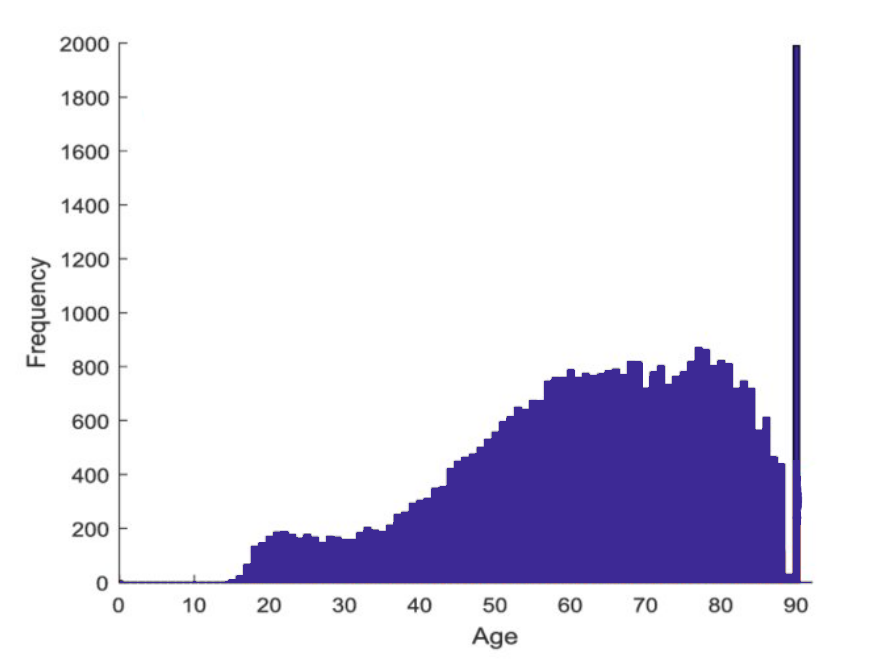
\includegraphics[width=8.5cm, height = 6cm]{ageDistribution.png}
    \caption{Age Distribution of MIMIC III}
    \label{age}
\end{figure}


\begin{table}[h]

    \caption{MIMIC III Statistics.}
    \label{statistics}
\begin{center}
\begin{tabular}{ | c | c | }
    \hline
 Number of patients     & 46520 \\ 
    \hline
 Number of Diagnoses    & 14567 \\  
    \hline
 Number of Procedures   & 3882 \\
    \hline
 Number of Procedures   & 4204  \\
    \hline
\end{tabular}
\end{center}

    \end{table}
